%% AZIENDA OSPITANTE
\chapter{Azienda ospitante}\label{chap:company}

\section{Profilo dell'azienda}
\begin{figure}[H] 
	\centering
	
\includegraphics[scale=0.3]{zextras}
	\caption{Logo Zextras s.r.l.}
	\label{fig:logoZextras}
\end{figure}
L'attività di stage descritta in questo elaborato è stata svolta presso l'azienda Zextras s.r.l. nella sede principale di Torri Di Quartesolo (VI). \\
La società è nata nel 2011 con l'obbiettivo di espandere le possibilità della \mmh{collaboration suite Zimbra}{cos'è? dico qui due paroline anche?}.
In pochi anni è riuscita a rendere la propria suite di prodotti l'estensione professionale per Zimbra Open Source più avanzata tra le soluzioni di collaborazione sul mercato. I loro prodotti sono riconosciuti come ottimali anche dalla \mmh{community Zimbra}{Avrà u nome no?} tanto che è in corso una collaborazione per lo sviluppo di alcuni prodotti open source e per Zimbra Suite Plus.
Ad oggi presenta uffici secondari in Francia, Brasile, Russia e negli Stati Uniti e possiede partner in tutto il mondo.\\
ciao

\subsection{Zimbra}
\begin{figure}[H] 
	\centering
	
\includegraphics[scale=0.2]{zimbra}
	\caption{Logo Zimbra}
	\label{fig:logoZimbra}
\end{figure}
Zimbra è un server di workgroup open source che mette a disposizione una suite di software collaborativi che consentono di condividere documenti e attività. 
Di base essa offre i seguenti servizi:
\begin{itemize}
	\item[•] configurazione personalizzata,
	\item[•] gestione della posta elettronica,
	\item[•] rubriche, calendari e condivisione di file,
	\item[•] chat e chiamate vocali,
	\item[•] integrazione con i canali web
	\item[•] privacy e alti livelli di sicurezza
	\item[•] disponibilità per i dispositivi mobili: oltre che mediante client Zimbra Web e attraverso i client di posta elettronica tradizionale, è possibile accedere alle e-mail, ai calendari e alle altre offerte da dispositivi mobile. 
\end{itemize}
Le funzionalità di Zimbra possono essere facilmente estese grazie alla possibilità di creare ed aggiungere degli add-on chiamati Zimlet. Esse sono delle integrazioni che permettono di personalizzare i servizi ed integrarli con servizi web e applicazioni di terzi.
Zimbra è disponibile in due versioni: 
\begin{itemize}
	\item Zimbra Open Source Edition: soluzione completamente open source ma con disponibili solo le funzionalità standard;
	\item Zimbra Network Edition: soluzione completa di tutte le funzionalità sia per l'amministratore di sistema sia per l'utente finale.
\end{itemize}


\subsection{Zextras Suite}
Zextras Suite è un Add-On per Zimbra Collaboration: i suoi prodotti sono progettati per espandere le funzioni di Zimbra Open Source Edition in maniera a se stante rispetto i moduli Zimbra Network Edition. Infatti Zextras Suite non è distribuito assieme ad alcun binario o sorgente sotto il copyright di Zimbra. \\
Le principali innovazioni che sono state portate nel mondo Zimbra riguardano la sicurezza dei dati, la mobilità e la gestione dello storage.\\
La suite comprende i seguenti prodotti:
	\begin{itemize}
		\item[•] Zextras Backup: un software che permette il backup in realtime e il ripristino per tutti i dati Zimbra;
		\item[•] Zextras Mobile: per sincronizzare le email, i contatti, gli eventi e ogni task con qualsiasi device mobile tramite Exchange ActiveSync;
		\item[•] Zextras Powerstore: per ottimizzare i volumi dei dati Zimbra e risparmiare spazio attraverso la compressione e la deduplicazione;
		\item[•] Zextras Admin: per monitorare gli utenti e le funzionalità di Zimbra, Zextras Suite e ogni altro Zimlet;
		\item[•] Zextras Chat: piattaforma client/server integrata in Zimbra per la messaggistica istantanea e le videochat.
	\end{itemize}

\begin{figure}[H] 
	\centering
	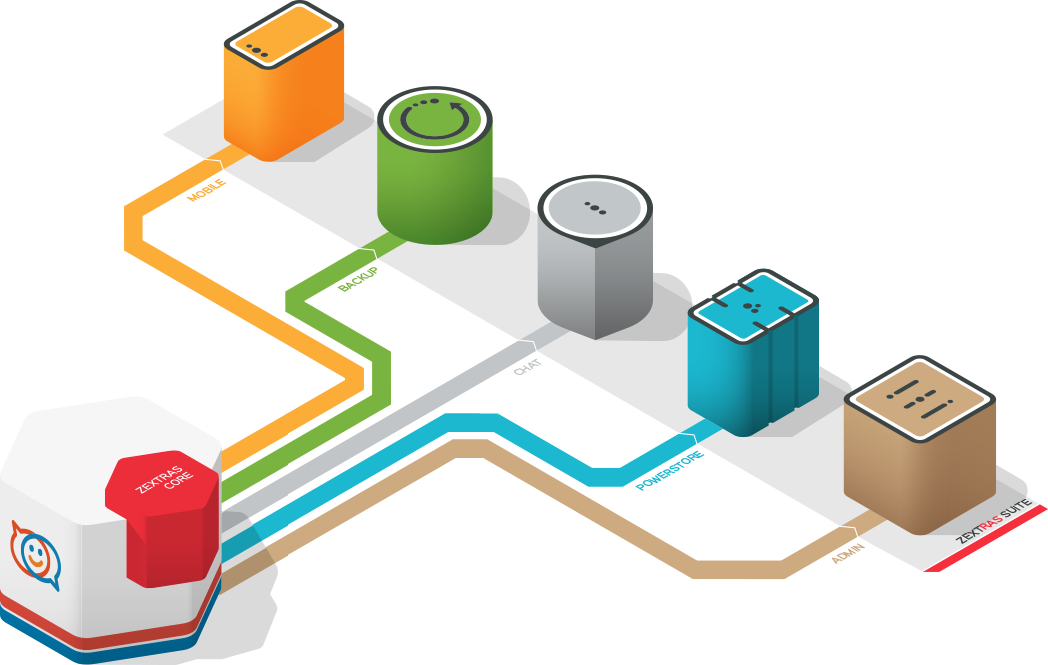
\includegraphics[scale=0.3]{zextras_2018}
	\caption{Rappresentazione Zextras suite}
	\label{fig:modulizextras}
\end{figure}
Come rappresentato in figura~\ref{fig:modulizextras}, Zextras suite è un'estensione modulare per Zimbra Open Source che può essere applicata secondo le proprie esigenze. Proprio per questo risulta la migliore scelta per un uso professionale di Zimbra.

\section{Metodo di lavoro}
\note{Il ciclo di sviluppo software adottato dall'azienda è un metodo agile...
Tecnicamente usano il metodo SCRUM, con la backlog e sprint di due settimane ...}

\subsection{Strumenti a supporto di processi e servizi}
\subsubsection{BitBucket}
\subsubsection{Jira}
\subsubsection{Bamboo}
\subsubsection{Confluence}

